\begin{frame}
\frametitle{Vertex Buffer: Demo}
\begin{figure}[ht]
    \centering
    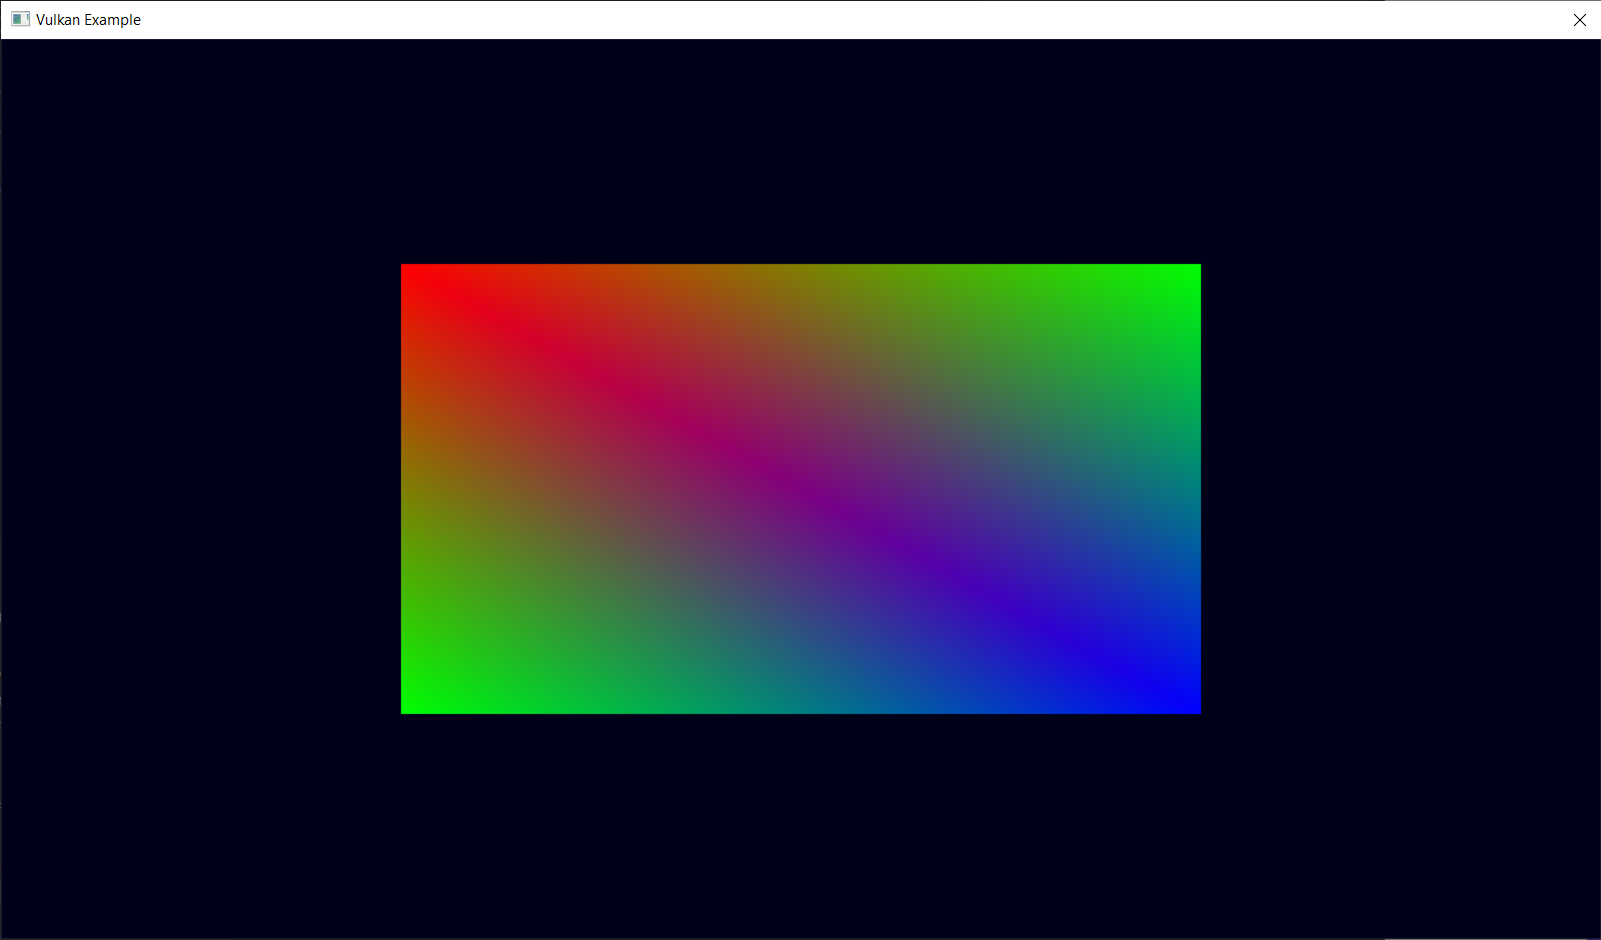
\includegraphics[scale=0.25]{images/SlidesVertices/RenderQuad.png}
\end{figure}
\end{frame}

\begin{frame}
\frametitle{Vertex Buffer}
\begin{itemize}
\item I dati dei nostri vertici sono in RAM e noi dobbiamo caricarli nella memoria della GPU
\item Usiamo due buffer
\item Uno staging buffer, allocato su memoria della GPU host visible
\item Scriviamo i dati dei nostri vertici su questo buffer
\item Un vertex buffer, allocato su memoria della GPU device local
\item Inviamo un comando che dice alla GPU di trasferire il contenuto dello staging buffer nel vertex buffer
\item Modifichiamo la creazione del nostro pipeline state object per specificare come interpretare i dati nel vertex buffer
\item Prima di registrare il comando per attivare la pipeline, registriamo un comando che indica alla pipeline grafica di usare come input il nostro vertex buffer
\end{itemize}
\end{frame}
